%==============================================================================
% Matt Nichols' Homework Template
%==============================================================================


%Fill out this line with the homework number
\newcommand{\visibleusernames}
{\space man1, malesser, ac110 }
{}
\newcommand{\thisclass}{CSCI 160}
\newcommand{\thishw}{Final Project}

%==============================================================================
% Formatting parameters
%==============================================================================

\documentclass[11pt]{article}			% 11pt article
\author{Matt Nichols}
\date{\today}
\makeatletter					% Make '@' accessible.

%Fill out this line with your name and login
\def\@oddhead{\bf \thisclass \space - \thishw\hfill \visibleusernames} % Here they are

\oddsidemargin=0in				% Left margin minus 1 inch.
\evensidemargin=0in				% Same for even-numbered pages.
\textwidth=6.5in				% Text width (8.5in - margins).
\topmargin=0in					% Top margin minus 1 inch.
\headsep=0.2in					% Distance from header to body.
\textheight=8.5in					% Body height (incl. footnotes)
\skip\footins=4ex				% Space above first footnote.
\hbadness=10000					% No "underfull hbox" messages.
\makeatother					% Make '@' special again.

%==============================================================================
% Packages used
%==============================================================================

\usepackage{amsmath}				% want AMS fonts
\usepackage{amssymb}
%\usepackage{psfig}				% want to include EPS files
\usepackage[pdftex]{graphicx}				% for including images
\usepackage{algorithmic}
\usepackage{algorithm}
\usepackage{hyperref}
\usepackage{tikz}


%==============================================================================
% Macros
%==============================================================================
\newcommand{\new}[1]{{\em #1\/}}		% New term (set in italics).
\newcommand{\set}[1]{\{#1\}}			% Set (as in \set{1,2,3})
\newcommand{\setof}[2]{\{\,{#1} $\mid$~{#2}\,\}}	% Set (as in \setof{x}{x > 0})
\newcommand{\N}{\mathord{\Bbb N}}		% Positive integers.
\newcommand{\compl}[1]{\overline{#1}}		% Complement of ...            
\newcommand{\bigand}{\bigwedge}
\newcommand{\bigor}{\bigvee}
\newcommand{\OR}{\vee}
\newcommand{\AND}{\wedge}
\newcommand{\code}[1]{\texttt{#1}}
\newcommand{\nlogn}{n \log n}

\newcounter{qcounter}
\setcounter{section}{0}
\def\thesection{Section \arabic{section}}


% \begin{list}{b\alph{qcounter}.}{\usecounter{qcounter}} <-- helpful

%==============================================================================
% Title
%==============================================================================

\begin{document}
\centerline{\bf \LARGE\thishw: Knock Detection Entry System}
\centerline{\today}

\section{Introduction}
 % Introduce your project. Succinctly explain your problem and solution. Why did you choose to work on it?
Carrying keys around has always been a hassle for all of us. If one loses a key, he or she has to be assisted by someone else to get in to the room. A lot of times, there are situations where you wouldn't want to bring your keys with you either, such as when you're going on a run.I personally have forgotten my keys in my room, or have been locked out by my roommate numerous times. We wanted an easier way to enter and exit a locked room, and not ever have to worry about being locked out. 
Our project is a reasonably straightforward Arduino program which enables pulling a doorhandle down from the inside of a door once a specific pattern of knocks has been detected. This pattern is configurable via a "record" function, and, when powered, the device is always listening for the pattern, ready to trigger a motor to open the door. If an incorrect knock pattern is given, the program alerts you through a buzz in the speaker. This way, the room is secure and you'll never be locked out because you don't have the key.

\section{Architecture}
% Describe the architecture of your system. Figures are welcomed and encouraged


\begin{center}
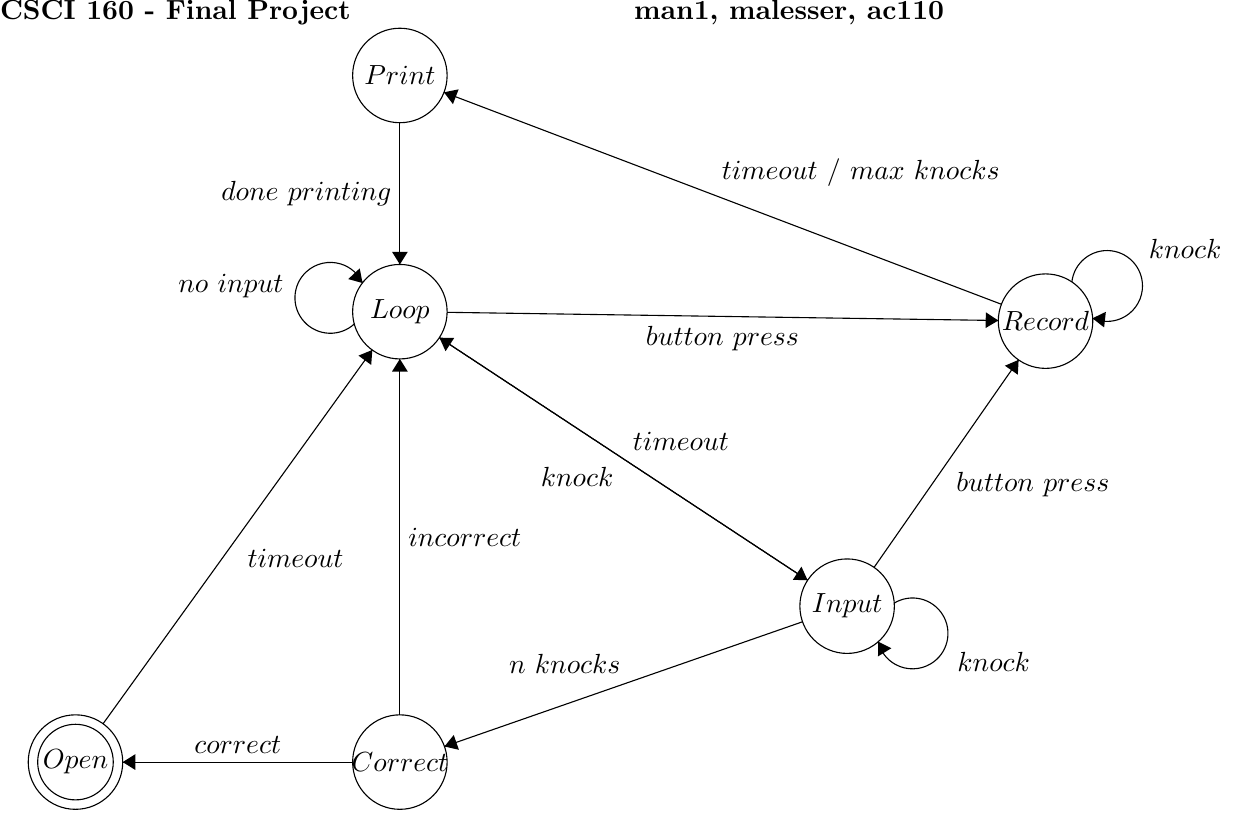
\begin{tikzpicture}[scale=0.2]
\tikzstyle{every node}+=[inner sep=0pt]
\draw [black] (26.6,-22.6) circle (3);
\draw (26.6,-22.6) node {$Loop$};
\draw [black] (55,-41.3) circle (3);
\draw (55,-41.3) node {$Input$};
\draw [black] (67.6,-23.2) circle (3);
\draw (67.6,-23.2) node {$Record$};
\draw [black] (26.6,-51.2) circle (3);
\draw (26.6,-51.2) node {$Correct$};
\draw [black] (6,-51.2) circle (3);
\draw (6,-51.2) node {$Open$};
\draw [black] (6,-51.2) circle (2.4);
\draw [black] (26.6,-7.6) circle (3);
\draw (26.6,-7.6) node {$Print$};
\draw [black] (29.6,-22.64) -- (64.6,-23.16);
\fill [black] (64.6,-23.16) -- (63.81,-22.64) -- (63.79,-23.64);
\draw (47.08,-23.48) node [below] {$button\mbox{ }press$};
\draw [black] (29.11,-24.25) -- (52.49,-39.65);
\fill [black] (52.49,-39.65) -- (52.1,-38.79) -- (51.55,-39.63);
\draw (37.85,-32.45) node [below] {$knock$};
\draw [black] (23.713,-23.373) arc (312.7283:24.7283:2.25);
\draw (19.24,-20.97) node [left] {$no\mbox{ }input$};
\fill [black] (24.23,-20.78) -- (24.05,-19.85) -- (23.32,-20.53);
\draw [black] (52.49,-39.65) -- (29.11,-24.25);
\fill [black] (29.11,-24.25) -- (29.5,-25.11) -- (30.05,-24.27);
\draw (44.45,-31.45) node [above] {$timeout$};
\draw [black] (52.17,-42.29) -- (29.43,-50.21);
\fill [black] (29.43,-50.21) -- (30.35,-50.42) -- (30.02,-49.48);
\draw (37.07,-45.62) node [above] {$n\mbox{ }knocks$};
\draw [black] (23.6,-51.2) -- (9,-51.2);
\fill [black] (9,-51.2) -- (9.8,-51.7) -- (9.8,-50.7);
\draw (16.3,-50.7) node [above] {$correct$};
\draw [black] (57.982,-41.109) arc (121.40093:-166.59907:2.25);
\draw (61.97,-44.82) node [right] {$knock$};
\fill [black] (56.97,-43.55) -- (56.96,-44.49) -- (57.81,-43.97);
\draw [black] (26.6,-48.2) -- (26.6,-25.6);
\fill [black] (26.6,-25.6) -- (26.1,-26.4) -- (27.1,-26.4);
\draw (27.1,-36.9) node [right] {$incorrect$};
\draw [black] (7.75,-48.77) -- (24.85,-25.03);
\fill [black] (24.85,-25.03) -- (23.97,-25.39) -- (24.78,-25.98);
\draw (16.89,-38.28) node [right] {$timeout$};
\draw [black] (64.8,-22.13) -- (29.4,-8.67);
\fill [black] (29.4,-8.67) -- (29.97,-9.42) -- (30.33,-8.48);
\draw (55.86,-14.69) node [above] {$timeout\mbox{ }/\mbox{ }max\mbox{ }knocks$};
\draw [black] (26.6,-10.6) -- (26.6,-19.6);
\fill [black] (26.6,-19.6) -- (27.1,-18.8) -- (26.1,-18.8);
\draw (26.1,-15.1) node [left] {$done\mbox{ }printing$};
\draw [black] (69.27,-20.722) arc (173.74488:-114.25512:2.25);
\draw (74.12,-18.63) node [right] {$knock$};
\fill [black] (70.58,-23.02) -- (71.32,-23.6) -- (71.43,-22.61);
\draw [black] (56.71,-38.84) -- (65.89,-25.66);
\fill [black] (65.89,-25.66) -- (65.02,-26.03) -- (65.84,-26.6);
\draw (61.9,-33.61) node [right] {$button\mbox{ }press$};
\end{tikzpicture}
\end{center}


\section{Implementation}
% Challenges, etc.

This program assumes a hardware configuration that includes a piezo element for knock sensing (connected on "piezo\_pin", in our code), two LEDs for control output, a button to trigger the recording mode, and a servo ("s1", connected on "servo\_pin") to pull the deadbolt.

The device begins with a default knock pattern of ten equally spaced knocks. In our system, a n knock pattern is represented as a n-1 sized array, each element being the ratio between adjacent knocks (so the default knock pattern is represented as [1, 1, 1, 1, 1, 1, 1, 1, 1]). When the system hears a first knock, it will begin recording the time offsets between subsequent knocks, and after a timeout (i.e. the knock has completed) relative ratios are calculated from the recorded offsets. Each of these ratios are then compared to those of the current key pattern (within an error margin), and if they all match then the servo is triggered and the deadbolt is pulled open.

Recording is very similar: pressing the button triggers record mode, and then the current key pattern will be replaced by whatever ratioed pattern is recorded after the button press (and before a timeout, as above). This pattern will then be played back to the user on a LED, and the device will re-enter normal operation, listening for entry attempts.

Installation: the device must be installed such that the piezo is pressed directly against the door, to best register knocking. The servo should be configured to pull the deadbolt out when it rotates (the user will need to handle re-locking the door).

Recording: press the button once, and then knock out the desired pattern on the inside of the door. Wait for the timeout, and then make sure the replayed pattern (on the second, lower LED) is as you desire. Your patterns must consist of between three and ten knocks (inclusive); shorter knocks will not overwrite the current key pattern, and recording will cut off after ten knocks.

Unlocking: simply knock the pre-recorded pattern on the outside of the door, and if the time ratios between your knocks match the stored key pattern, the servo will pull the deadlock. It must be manually re-locked afterwards. If you make a mistake in the pattern, wait four seconds (the timeout) and try again.

\section{Evaluation}
% did it work? Are there any corner cases? How would you solve them?
Yes it did work. 

\section{Related Work}
% Are there any similar solutions? Compare yours to theirs, if possible.
There aren't many similar affordabe solutions. Doors with fingerprint scanners exist but are extremely expensive, even though they're more secure. "The Clapper" also exists, that gives current to an outlet if it detects claps. However, it doesn't let you customize the sequence of claps. It doesn't directly connect to a motor either. Lastly, it detects sound as a pose to vibrations. Our project won't detect random noises, only vibrations on the door whereas "The Clapper" could interpret white noise and randomly open and close the door.

\section{Future Work}
% Describe here features that you wanted to implement, but due to time/resource constraints you weren't able to.

In the remote\_unlock/ directory of the repo, we have the backend/server script for implementing SMS-triggered unlocking as well (via Twilio). Alas, we haven't yet had any successes in configuring the device's side of this functionality; however, should the device be configured with an ethernet shield, it would be simple to poll against [server port]/state and trigger the servo when the "Unlocked" state is observed.

\end{document}